\documentclass[10pt, twocolumn]{article}

\usepackage{fullpage}
\usepackage{amsmath}
\usepackage{amsthm}
\usepackage{url}
\usepackage{relsize}
\usepackage{xspace}
\usepackage{subfigure}
\usepackage{graphicx,color}
\usepackage{amssymb}
\usepackage[margin=0.82in]{geometry}

%\setcounter{secnumdepth}{2}

\def\TODO#1{\noindent\textbf{[TODO:} #1]}

\begin{document}
\title{Predicting the Stock Market from History and Newspaper Articles \\ \begin{large}6.867 Machine Learning Course Project\end{large}}

%\subtitle{6.867 Final Project}
\author{Christopher R. Johnson  \\ \texttt{crjohns@mit.edu} \and Fredrik Kjolstad \\ \texttt{fredrikk@mit.edu}}
\date{December 10, 2012}
\maketitle

\begin{abstract}
\end{abstract}

\section{Introduction}

\TODO{Describe how we took an exploratory approach with made us end up with many classifiers. That is, we tried simple classifiers first and moved on to more sophisticated classifiers when we were not happy with our results.}

\begin{figure}
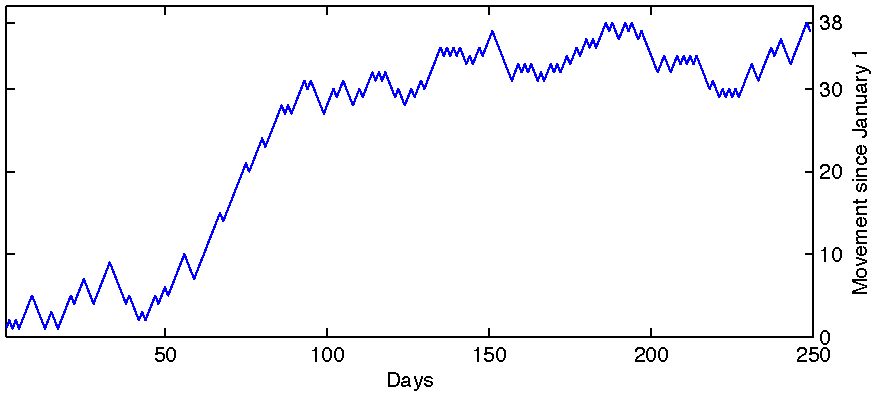
\includegraphics[width=8.5cm]{experiments/dj_performance.pdf}
\caption{Dow Jones movement from January 1 to December 31 2007. The Y axis shows cumulative movement since January 1.}
\label{fig:dj-preformance}
\end{figure}

\TODO{Motivate the problem and explain the different market hypotheses in \cite{mlstockmarket}}

\subsection{Related work}
\cite{twitter}, \cite{mlstockmarket}

\section{Feature Selection}
\label{sec:features}

Our data set consists of 36,466 Wall Street Journal (WSJ) articles over 359 days, and 251 days of closing price information of the Dow Jones Industrial Average (DJI) for the year 2007. The stock market is closed on weekends and holidays, which is why there are fewer days of stock data than newspaper articles. There are two days for which we have stock data but no newspaper articles (December 18th and 27th), but this appears to be an omission in the provided data set. We consider only days for which we have both WSJ and DJI data. This includes omitting data from weekends, which may be too strong a simplifying assumption.

\TODO{We need to mention weekends, but this might be too negative}

We have approximately 101 articles per day on average. A histogram of articles per day appears in Figure~\ref{articlehist}. The distribution appears to be bimodal, with numbers of articles around either 125 or 15 per day. Some days have fewer articles, which may decrease their effectiveness for classification. In Section~\ref{sec:bagsofwords} we mention some strategies used to scale the counts so that effects of this difference may be reduced.

\begin{figure}
\centering
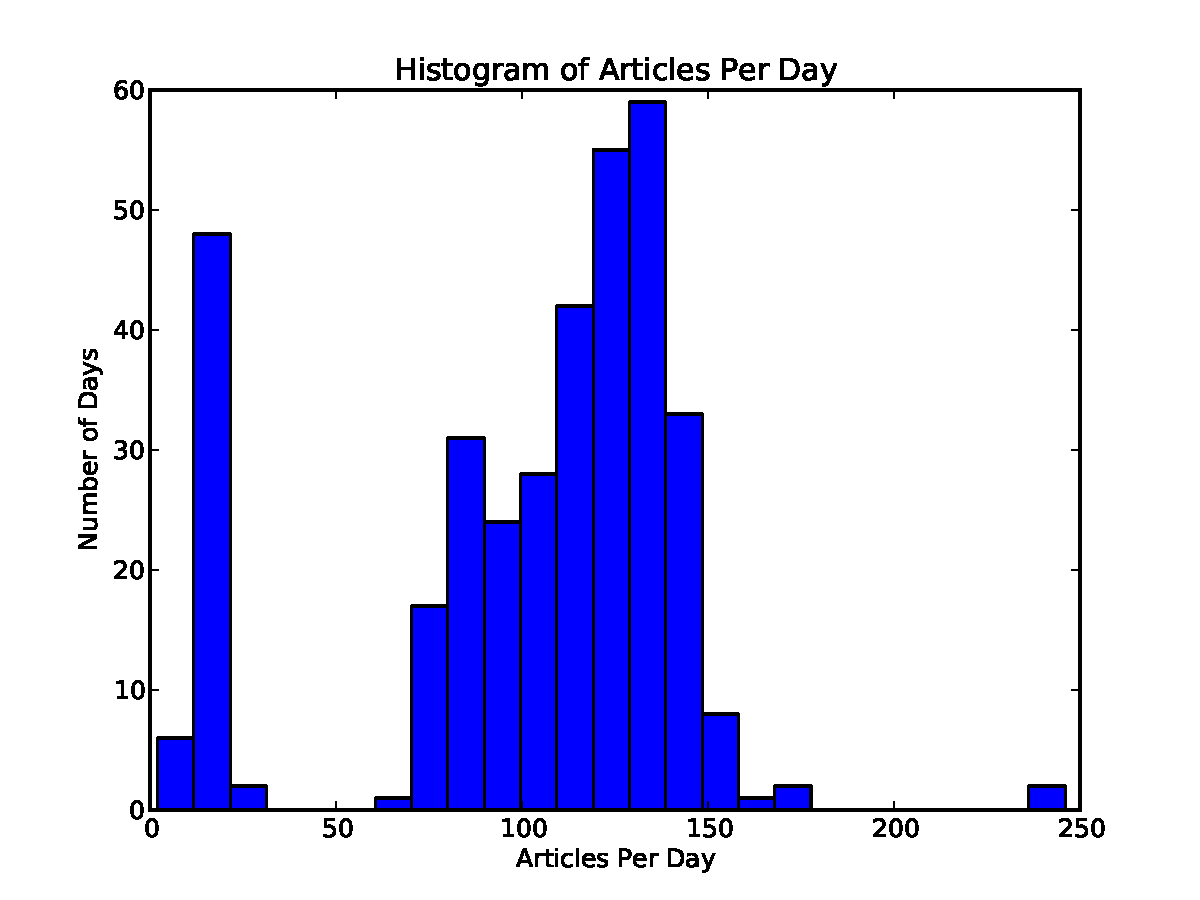
\includegraphics[scale=0.3]{text/articleshist.pdf}
\caption{Histogram of Articles Per Day}

\label{articlehist}
\end{figure}

Our data set consists of over 24 million words, with an average of 667 words per article. A histogram of article lengths appears in Figure~\ref{wordshist}. Most articles tend to be less than 2000 words, but there appears to be a long tail consisting of a few very long articles. For the most part it appears that article lengths are similar apart from a few outliers.


\begin{figure}
\centering
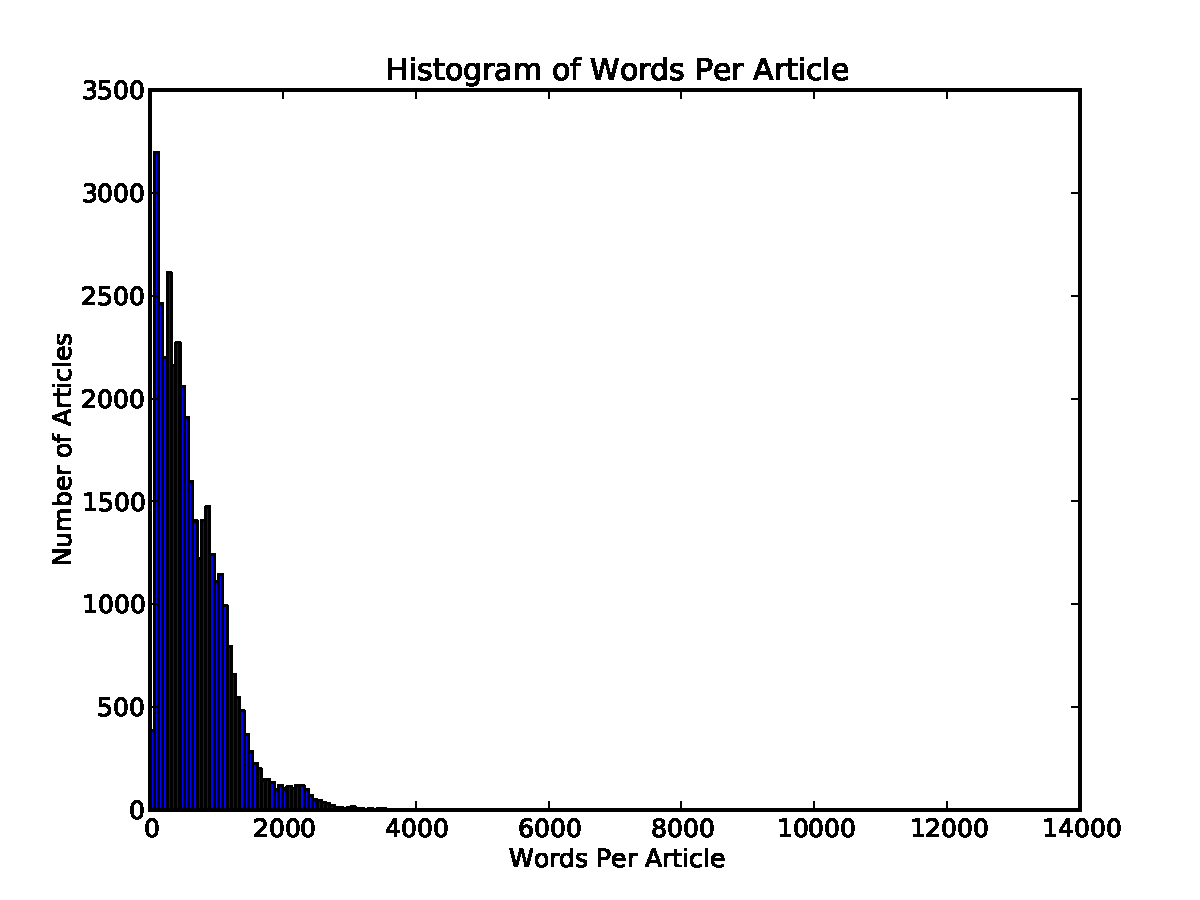
\includegraphics[scale=0.3]{text/wordshist.pdf}
\caption{Histogram of Words Per Article}
\label{wordshist}
\end{figure}

The data set contains 150,875 unique words. Each data point we use for training and validation therefore consists of a class label (+1 if the market went up that day, -1 if it went down) and a feature vector computed using frequencies of these unique words.

Due to the difficulty of computation on the number of unique words that we have, we filter the words in several ways to reduce the noise of the data set. First, we strip all non-alphabetic characters from all words and filter out any words less than length 2. We then filter out any words that did not appear more than some cutoff, $m$, throughout the year. We assume that these words are either misspellings or words which would not generally be useful in predicting stock performance due to their infrequency. Filtering with $m = 10$ results in 44,218 unique words and was found to be a good balance between information and computational tractability.
Finally, we filtered out any of the 100 most commonly used English words~\footnote{http://en.wikipedia.org/wiki/Most\_common\_words\_in\_English}, since we
assume that words such as ``and'' and ``I'' do not provide very much information.

We use several feature extraction techniques to construct the data matrix $F$. Each row of $F$ is the feature for a corresponding day, and each column of $F$
contains the values for one feature across all days. The column-vector $Y$ contains the output values (+1 or -1). 

The rest of this section describes several feature extraction techniques we used and the representation of the feature matrix $F$.  These features are compared using several machine learning algorithms presented in Section~\ref{sec:techniques}.

We will introduce the following terminology to describe the feature matrix and its elements:

\begin{itemize}


\item $F_{d,i}$ is the ith element of the feature vector for day $d$.

%\item $W$ is a vector with a count for each word over the entire year. Thus, $W_i$ is the number of times word $i$ appeared in the year.  

\item $A$ is a vector of word counts for a single article. Thus, $A_i$ is the number of times word $i$ appeared in article $A$.

\item $D$ is a vector of days, each element of which is a set of articles. $A \in D_k$ if and only if article $A$ was published on day $k$.


\end{itemize}

\subsection{Bag of Words and Phrases}
\label{sec:bagsofwords}

The simplest feature vector is simply a ``bag of words'' for each day~\cite{featurehash}, which consists of frequency counts of all words in articles published on that day. Elements of the feature vector take the form: $$\displaystyle F_{d,i} = \sum_{A \in D_d}{A_i}$$ These feature vectors are extremely sparse, since most articles do not use tens of thousands of unique words (we represent our data set as a sparse matrix
in MATLAB to reduce memory consumption to reasonable levels).

An obvious weakness of this technique is that it takes words out of context. Phrases such as ``stocks went up'' simply increase the counts of the three words independently. We augmented this technique by creating ``bags of phrases'' as well. In addition to counts of words, we keep counts of two and three word phrases
as well. We turn phrases into single words of the form ``word1-word2'' and ``word1-word2-word3'' with the restrictions that word1 and word3 may not be common words and the first or last words of a phrase may not be a single character. Common words beginning a 2 word phrase or ending a 3 word phrase are undesirable because we want to pick up on phrases where the subject is important. The middle word in the 3 word phrases may be common so we find phrases that combine two useful words such as, ``stocks are down.'' Filtering out phrases that appear less than $m = 10$ times in the year results in 194,679 unique words and phrases, so this technique can greatly increase the number of features. When using phrases, we instead filter out words and phrases that appear less than $m = 50$ times in the year, leaving us with 37,904 words and phrases. 

A bag of words for each day has several other problems. First, it reduces all articles for a single day to a bag of words for that day, potentially losing some information. Computing on counts of words per article per day would quickly become intractable in terms of memory consumption, so this simplifying assumption was necessary to compute on the data. Another problem is that some days have fewer articles than other days, which is a source of variation in the data which we do not wish to measure. We can condition our data to replace each word count with the proportion of times that word appears out of all words in the day, and we evaluate the effect of this conditioning later on SVMs and K-Nearest-Neighbor methods which may benefit from it. This kind of conditioning is unnecessary for Naive Bayes.

Bags of words and bags of phrases form the basis of many of our other feature selection techniques, so we will call the feature matrix resulting from the use of either $B$. Since bags of phrases just increase the vocabulary size, it can be viewed as augmenting the article word lists $A$ with additional words. The bags of words or phrases may be used interchangeably, so we will refer to the resulting feature matrix for either as $B$ in the rest of this section; when we present results we will explicitly state if we build on bags of words or phrases as well as the filtering parameters used.

As mentioned previously,

\subsection{Temporal Features}

The words and phrases from previous days may have an influence on the current day's market direction by representing trends in the market~\cite{mlstockmarket}. Building a model which takes temporal information into account may use information about these trends to make better predictions. We incorporate temporal information by augmenting our data set with data from previous days and using the resulting feature vectors for training and testing.

The first method we consider is \textit{temporal concatenation} of our bag of words. The previous $L$ days features are concatenated on to the end of the current day's feature. That is, $F_{d} = B_{d} \oplus B_{d-1} \oplus ... \oplus B_{d-L}$, where ($\oplus$) represents vector concatenation, and where days before the start of our data set are assumed to have counts $0$ for all words.

A major problem with this method is that it increases the length of our feature vectors by a factor of $L$, which quickly becomes intractable for large $L$. To use this method, we need to filter out more words from our initial data set which may reduce the information we have. Another problem with temporal concatenation is that it also includes information about which specific day in the past had each word. If the phrase ``market downturn'' is associated with decreases in the following week, then it doesn't matter if it appeared one or two days in the past. This observation is similar to that made in~\cite{mlstockmarket} in which the author assumes that certain articles may have an effect on the stock price that lingers for some time and then diminishes in importance. 

The second method we consider, which we call \textit{temporal memory}, addresses this issue. Each feature vector is augmented with a weighted average of the frequencies of each word over the previous $L$ days. That is, $$\displaystyle F_{d} = B_{d} \oplus {{\sum^L_{i=1}{\alpha_i B_{d-i}}} \over {\sum^L_{i=1}{\alpha_i}}}$$ Again, frequencies are assumed to be 0 for days before the beginning of our data set, and we round the weighted average up to an integer. This allows us to specify the relative weights of historic data for the previous $L$ days while only doubling the size of our feature vectors. 

\subsection{Topic Modeling and Dimensionality Reduction}
\label{sec:topicmodel}

The feature vectors previously described in this section are all very high-dimensional, containing either tens- or hundreds-of-thousands of word frequencies. This is problematic for several learning algorithms we applied, including SVMs and K-Nearest-Neighbor. We use dimensionality reduction and topic modeling techniques to reduce the dimensionality of the feature vectors while retaining important semantic information.

The primary technique we use is Latent Semantic Indexing~(LSI)~\cite{lsi}. The input to LSI is a term-document matrix, a matrix in which each row represents a term and each column represents a document. The element at row $t$ and column $d$ is the frequency of term $t$ in document $d$ (this is the transpose of our bag of words feature matrix $B$, viewing each day as a ``document''). LSI requires finding the Singular Value Decompositon (SVD) of this term-document matrix. If $X$ is our $t \times d$ term-document matrix, then the SVD of $X$ are the unique matrices $T, S, \text{ and } D$, such that $T$ is $t \times m$, S is diagonal $m \times m$, $D$ is $d \times m$ and $X = T S D'$, where $D'$ is the transpose of $D$. By the definition of SVD, the columns of $T$ are eigenvectors of $X X'$, the rows of $D$ are the eigenvectors of $X' X$, and $S$ is a diagonal matrix of the square roots of the eigenvalues for both. The fundamental insight used by LSI is that zeroing out all but the $r$ largest eigenvectors in $S$ results in a new matrix $\hat{X}$ which is the closest matrix of rank $r$ to the original $X$ by least-squares~\cite{lsi}. Zeroing out those elements also means we need to retain only $m$ columns of $T$ and $D$ to construct the new matrix, so we have greatly reduced the number of columns we must retain for $r << m$. This result is called the rank-reduced SVD. The $r$ columns of $D$ corresponding to the $r$ largest eigenvalues represent each document with only $r$ features, multiplying by $S$ scales this new vector space appropriately, so we use $S D'$ as our data matrix which is $d \times r$ with similarity between vectors representing similarity between semantic information in the original input space. The LSI paper recommends finding similarity by cosine of the angle between vectors, and we compare using angle and Euclidean distance in our results. New input vectors can be projected into this new space through a method described in~\cite{lsi}.


\begin{figure}
\centering
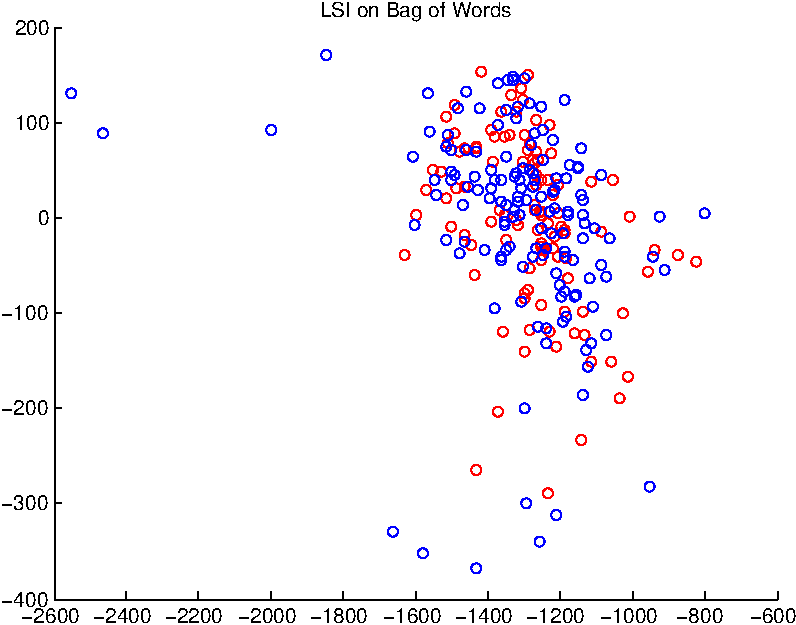
\includegraphics[scale=0.4]{plots/lsiorig.pdf}
\caption{Feature space from 2D LSI on the original bag of words}
\label{lsiorig}
\end{figure}

\begin{figure}
\centering
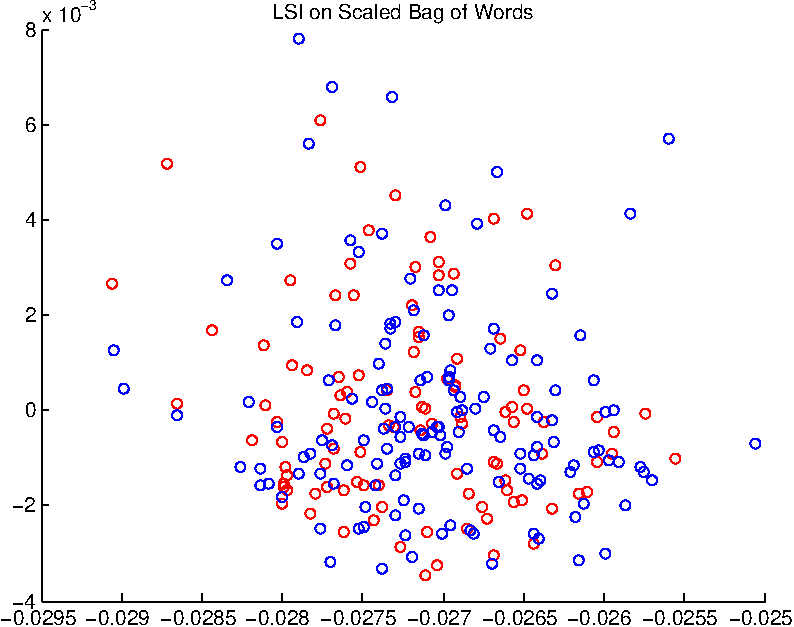
\includegraphics[scale=0.4]{plots/lsiscaled.pdf}
\caption{Feature space from 2D LSI on the scaled frequencies of words each day}
\label{lsiscaled}
\end{figure}

\begin{figure}
\centering
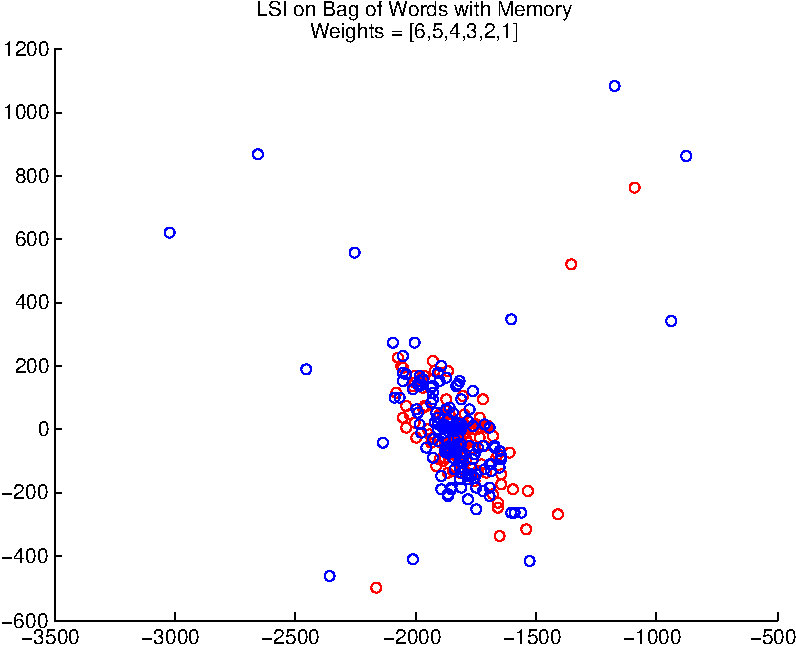
\includegraphics[scale=0.4]{plots/lsimem.pdf}
\caption{Feature space from 2D LSI on data augmented with 6 days of memory}
\label{lsimem}
\end{figure}

\begin{figure}
\centering
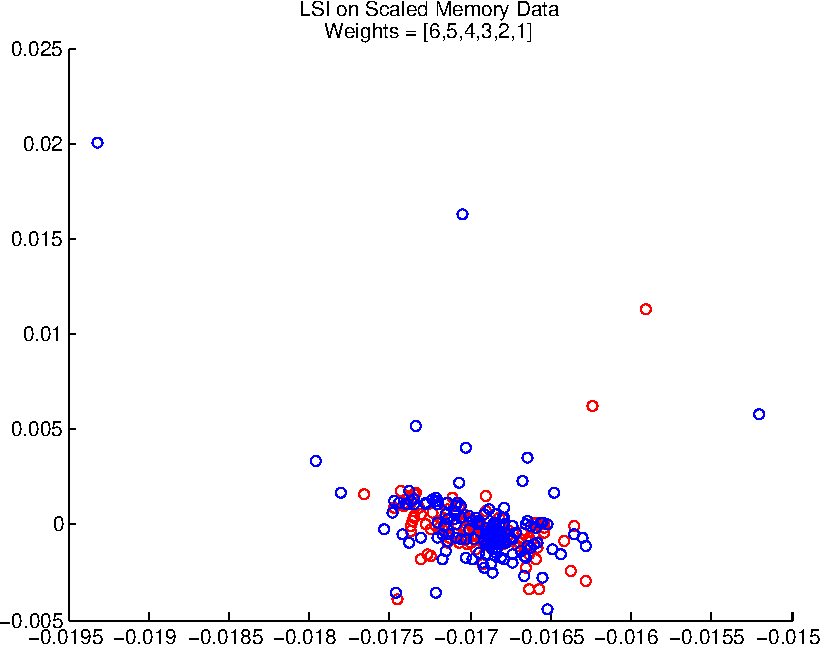
\includegraphics[scale=0.4]{plots/lsimemscaled.pdf}
\caption{Feature space from 2D LSI on data augmented with 6 days of memory, which was then scaled}
\label{lsimemscaled}
\end{figure}

\begin{figure}
\centering
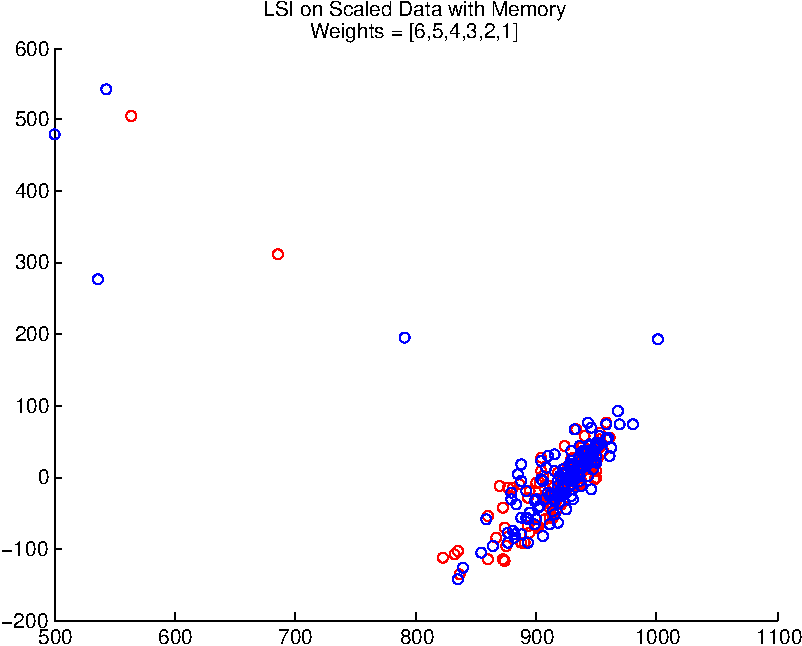
\includegraphics[scale=0.4]{plots/lsiscaledmem.pdf}
\caption{Feature space from 2D LSI on scaled data augmented with 6 days of scaled frequencies}
\label{lsiscaledmem}
\end{figure}

Figures~\ref{lsiorig},~\ref{lsiscaled},~\ref{lsimem},~\ref{lsimemscaled},~and~\ref{lsiscaledmem} show different vector spaces resulting from running LSI and reducing to two dimensions for data conditioned using several previously mentioned techniques. The red circles are feature vectors for days the market went down, and the blue circles are feature vectors for days the market went up. A reduction to two dimensions loses a lot of data, but it allows us to graphically investigate the structure of our data resulting from initial feature choices and LSI itself. In later experiments we will reduce the space to approximately 100 features as recommended in the literature~\cite{lsi}.  

The initial observation from all of the Figures was that the data is not linearly separable in two dimensions. This is expected, since that would imply a very strong relationship between articles and closing stock prices and would make stock prediction trivial. Certain techniques such as hard-margin SVMs will not work, so we will look to evaluate these features using soft-margin SVMs and K-Nearest-Neighbors in later sections. Figures~\ref{lsiorig}~and~\ref{lsiscaled} demonstrate the effect of scaling on our resulting feature space. Applying LSI to the original bag of words has a large mixed cluster of up and down days, along with several outliers that are mostly up days. Applying LSI to the scaled bag of words results in a more centered data distribution with some areas of higher ``up'' density. The data is slightly better clustered, but it is still very noisy and may be difficult to use for good predictions. Figures~\ref{lsimem},~\ref{lsimemscaled},~and~\ref{lsiscaledmem} show the effects of augmenting with a weighted average 6 days of temporal data. The difference between Figures~\ref{lsimemscaled}~and~\ref{lsiscaledmem} is that Figure~\ref{lsimemscaled} shows the result of first augmenting $B$ with temporal data and then scaling it, while Figure~\ref{lsiscaledmem} shows the result of scaling $B$ and then augmenting that with a weighted average of 6 days of scaled word frequencies. The three figures show densely clustered data with several sparse outliers. The dense clustering may be the result of most days having similar histories. The outliers are, interestingly, mostly up days. This may be detecting long term trends in the newspaper and the market. Figure~\ref{lsiscaledmem} interestingly has a long tail out to the positive $x$ direction while it has a lot of variance in the $y$ direction for $x$ values around $-125$. This is mostly an artifact of the scale of the graph, looking at the $y$ scale it is clear that the region of high $y$ variance has about as much variance in the $x$ direction. The top and bottom of this distribution, however, have many up days, which may be useful for classification.

\TODO{Look through data sets and explain some outliers}

LSI clusters documents by projecting them to a lower-dimensional space and using a distance metric to measure similarity between topics. We briefly investigated using Probabilistic Latent Semantic Indexing (PLSI) to model topics and reduce the dimensionality differently~\cite{plsi}. PLSI addresses LSI's lack of a solid statistical model by modeling the distribution on terms, documents, and latent ``topics'' of those documents in the graphical model represented in \TODO{show figure here}. The model can be trained to fit $k$ topics to the data by the EM algorithm, and the posterior probabilities of topics can be computed to classify the input. We planned on using this to classify documents appearing each day, and reducing the dimensionality of the feature vectors to be a count of topics appearing during the day rather than a count of words. We implemented the PLSI algorithm iteratively, but PLSI appears to be intractable even on a small subset of our data set due to the high number words within those documents. We could remove some articles from the data set to make it more tractable, but we would lose a lot of information in doing so. We opted instead to simply use LSI which can incorporate all of the data efficiently. Also related is Probabilistic Dirichlet Allocation, which extends PLSI with a Dirichlet prior on words and documents~\cite{lda}, but that technique is beyond the scope of this project.

\section{Classifiers}
\label{sec:techniques}

In this section we describe the different classifiers we developed for this project.
For each classifiers we describe our implementation choices and what, if any, third-party libraries we used.
We implemented all of our classifiers as MATLAB functions.

Our classifiers can roughly be divided into four categories. The first are simple prediction rules. These are mostly included to demonstrate features of our data and to serve as baselines for the other classifiers. The next class include classifiers that do not have a probabilistic model. These include AdaBoost, Nearest Neighbor and SVM. The third class consist of classifiers based on probabilistic models. The only classifiers we implemented in this category is Naive Bayes. The fourth and final class of classifiers is sequential models and include M-order Markov Models and Hidden Markov Models.

\subsection{Naive Bayes}
\label{sec:naive-bayes}

The first classifier we implemented was Naive Bayes.
Naive Bayes is a natural choice when the input features are discrete with very high dimensionality, which is the case with our bags of words and phrases.
The reason for this is the naive bayes assumption, which asserts that the input features are independent given the class.
This means we can turn the multinomial on the full distribution, which has $O(2^D)$ parameters into $D$ binomials with $O(D)$ parameters.
That is, $p(Y|X) \propto p(Y)p(X|Y) = p(Y)\prod_{i=1}^{D}{p(X^{(i)}|Y)}$, where $p(Y)$ is a prior on $Y$ (we will take advantage of the opportunity to put a prior on $Y$ later).

Although this assumption may seem \emph{overly} naive, it has proven to work well on document classification tasks such as spam detection, which are similar to our problem.
It is also a probabilistic model, as opposed to most of our other classifiers, which means we can combine it with temporal probabilistic models.

\subsection{AdaBoost}
\label{sec:adaboost}

The next classifier we implemented was AdaBoost using decision stumps as weak learners.
Our implementation of AdaBoost is parameterized by $M$, which denotes the number of classifiers to train.

The reason why we choose AdaBoost is that we have a very large corpus of words and need classifiers that can be trained very quickly.
Weak learners fit this bill since they can be trained in linear time in the dimensionality of the features and in the number of data points.
However, since decision stumps are terrible classifiers we boost them with AdaBoost, which makes them quite effective classifiers.
Moreover, in addition to serving as a efficient classifier on bags of words, AdaBoost helps us gain insight into our data set as the training picks out the words that does the best job of separating the dataset.

\subsection{Nearest Neighbor}
\label{sec:nearest-neighbor}

We implemented K-Nearest-Neighbor using feature vectors processed using LSI as decribed in Section~\ref{sec:topicmodel}.

Since LSI reduces the dimensionality of the feature space to identify latent features, we project input feature vectors into the training space and take the majority vote of the $k$ points in the training set closest to the new point under some metric. We use both angle (as used in~\cite{lsi}) and Euclidean distance.

\subsection{Support Vector Machine}
\label{sec:svm}

We used our implementation of dual form kernalized Support Vector Machines (SVM) with slack variables from a previous assignment.
This implementation uses the MATLAB quadprog function to solve the resulting quadratic optimization problem.
Our implementation is parameterized by $C$, which represents the weight given to the slack variables in the optimization problems. Higher values of $C$ give a harder margin SVM, but they tend to generalize worse.

Since it doesn't make sense to train an SVM on a bag of words, we use the feature vectors resulting from LSI as described in Section~\ref{sec:topicmodel}.

\subsection{Sequential Models}
\label{sec:sequential-models}

Stock Markets are known to follow trends and previous results are an often an indication of future results.
Therefore, we experimented with two sequential models to attempt to predict the Dow Jones based on past performance.

The basic versions of these models only use the previous history of Dow Jones performance to predict future results, and ignores the issues of the Wall Street Journal.
However, we also combined Hidden Markov models with Naive Bayes in an attempt to improve our predictions by taking more information into account.

\subsubsection{Markov Models}
\label{sec:mm}

We implemented M-order Markov Models for any value of M. However, since the number of model parameters grows exponentially in M, we are restricted to relatively small values of M by computational resources.

\subsubsection{Hidden Markov Models}
\label{sec:hmm}

We also implemented a classifier for the more powerful Hidden Markov Models. An HMM assumes the observed values $Y$ are generated from a sequence of hidden states $Z$.
The evolution of the hidden states is governed by the conditional probability distribution $p(Z^{(i)}|Z^{(i-1)})$ and the values of $Y_{i}$ are governed by the conditional probability distribution $p(Y^{(i)}|Z^{(i)})$.
%This is depicted graphically as a Bayes Net in figure~\TODO{ref}.

The HMM classifier is trained using the values $Y^{(1)}...Y^{(t-1)}$ and then used to predict value $Y^{(t)}$.
We used the MATLAB HMM Toolkit to learn the maximum-likelihood estimation of the model parameters A (the transition matrix) and B (the emission matrix) using the hmmtrain function, which internally uses the EM algorithm.
We then used the function hmmdecode to generate the posterior probability on state $Z^{(t-1)}$.
We then performed standard message passing along the chain from $Z^{(t-1)}$ to $Y^{(t)}$ to evaluate the marginal $p(Y^{(t)})$, which we used to predict $Y^{(t)}$.
Figure~\ref{fig:hmm-predict} illustrated this model.

\begin{figure}
\center
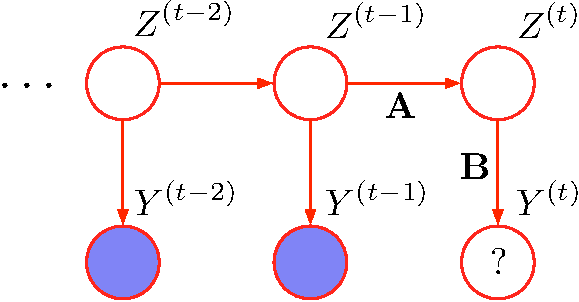
\includegraphics[width=6cm]{figs/hmm-predict.pdf}
\caption{Predicting the movement of the Dow Jones on day $t$ ($Y^{(t)}$) using a Hidden Markov Model to model trends in past performance.}
\label{fig:hmm-predict}
\end{figure}

In a variation on this approach we combined the Hidden Markov Model with Naive Bayes to make prediction both based on trends in the market and based on the articles in the Wall Street Journal.
To do this we first evaluated the marginal $p(Y^{(t)})$ as described above.
We then trained a Naive Bayes predictor on the first $t-1$ tuples, $\{(X^{(1)},Y^{(1)}), ..., (X^{(t-1)},Y^{(t-1)})\}$, and used this to predict the value of $Y_{t}$, using marginal $p(Y_{t})$ from the HMM as a prior.
That is, we combine our prior belief about which way we think the market will go based on recent performance, with the new information in the WSJ.
This is illustrated in figure~\ref{fig:hmm-nb-predict}. 

\begin{figure}
\center
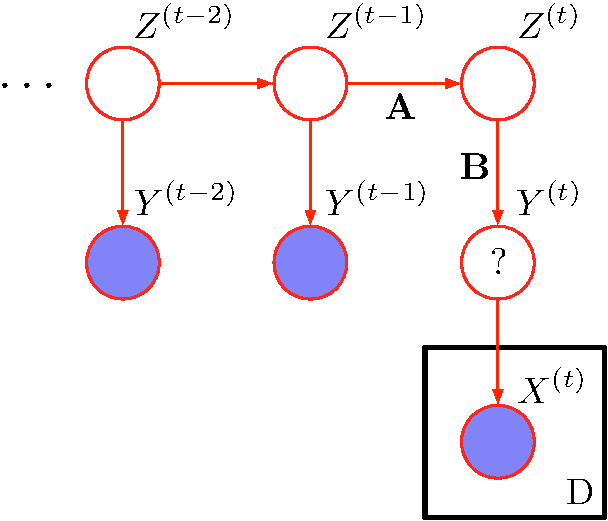
\includegraphics[width=6cm]{figs/hmm-nb-predict.pdf}
\caption{Predicting the movement of the Dow Jones on day $t$ ($Y^{(t)}$) using a Hidden Markov Model to model trends in past performance, combined with Naive Bayes to incorporate information in the Wall Street Journal.}
\label{fig:hmm-nb-predict}
\end{figure}

\section{Evaluation and Analysis}

In this section we seek to answer the following research questions:
\begin{description}
\item[Question 1] Can we predict the movement of the Dow Jones based on the Wall Street Journal?
\item[Question 2] Can we predict the movement of the Dow Jones based on past performance?
\item[Question 3] Can we predict the future performance of the stock market to make money?
\end{description}

The following subsections seek to answer these questions through a series of experiments that employ our suite of classifiers and feature sets.
In Section~\ref{wsj->dj} we address question 1 using non-sequential classifiers.
Section~\ref{dj->dj} addresses question 2 using both non-sequential classifiers with temporal features and sequential models such as Markov Models and Hidden Markov Models.
We address question 3 in both Section~\ref{wsj->dj} and Section~\ref{dj->dj} in terms of their respective models.
In both sections we analyze whether we can make money this way and hence whether this is a worthwhile pursuit.
Along the way we use our findings to gain insight into the underlying model and our data sets, and we use these insights to guide our search for the universal Dow Jones Predictor\footnote{Also known as our tropical island retirement plan: Happyface. Or not: Sadface.}.


\subsection{Predicting the Dow Jones based on the Wall Street Journal}
\label{wsj->dj}

\TODO{Chris: Use the models from section 4.1 to predict December. Add a section at the end for this}
\TODO{Add two sentences about the baseline at the beginning.}
\TODO{Rephrase hypothesis in terms of research question 3. 1 is predicting at all. 3 is predicting in such a way as to make money.}

The first question we wish to answer is whether we can find correlations between words in the Wall Street Journal and the Dow Jones, and use these correlations to classify days as ``up days'' or ``down days.'' We use several different feature vectors under each of our non-sequential models to test two hypotheses. First, we test that we can use some features of the data set to classify each day with a high degree of accuracy. Second, we test that can use feature vectors derived from days occuring before a given day to classify that day and therefore predict the direction of the stock market.

The first feature sets that we consider are bags of words (or phrases) associated with each day, and we attempt to classify the days using algorithms that work well on bags of words, namely Naive Bayes and AdaBoost. For training and verification, each day uses as data a bag of words from either the previous day (yesterday), the same day (today), or the next day (tomorrow). We therefore are attempting to classify each day using the previous day's articles, the same day's articles, or the next day's articles. Obviously, classifying a day based on the next day's articles is not useful for prediction, but it does allow us to investigate our first hypothesis (that we can find any correlation between the market and the newspaper at all), since it is reasonable to believe that the newspaper on the next day would have some mention of the stock market performance. The other features test how well we can predict the market. We also include bags of words for the current day augmented with the bag of words for the previous day, by the method described in the previous section.

To evaluate our predictors we used k-fold cross validation and split the data set into 12 equal sized sets, each of which would be chosen independently to be the verification set while the rest were used for training. The results in this section are from using k-fold validation on a fixed permutation of the data. For model selection we may want to randomize the arrangement of the data each time, but this section focuses on comparing the different methods and using a fixed permutation of the data allows for more direct comparison since the validation sets will remain consistent across tests.

\begin{table}[h]
\centering
\begin{tabular}{|l|l|l|} \hline
Data Used & Bag of Words & Bag of Phrases/Word \\ \hline
yesterday & 51.46\% & 52.58\% \\
today & 52.71\% & 53.84\% \\
today-aug & 51.46\% & 52.05\% \\
tomorrow & 51.98\% & 58.33\% \\ \hline
\end{tabular}
\caption{Naive Bayes comparison on several different features vectors.}
\label{tab:nbcompare}
\end{table}

The results from k-fold validation of Naive Bayes on these different data sets appear in Table~\ref{tab:nbcompare}. Some interesting trends appear in this data. First, the words from a given day predict that day better than articles from the previous day. Second, bags of phrases perform better than bags of words in all cases. The additional contextual data seems to aid prediction even though it meant leaving out many words. Augmented data including the previous day did not perform as well as just using the current day's articles. This could just be due to the increased sparsity of the data under augmentation. In terms of our second hypothesis, we gain some information about the future of the stock market based on previous articles. The proportion of positive days is 57.43\%, so given our results the predictive power of articles may be weak. In terms of our second hypothesis, it is clear that we gain some information about a day's stock price given the next day's newspaper. This seems to support our hypothesis that we can classify the days based on only the newspaper.

\begin{table}[h]
\centering
\begin{tabular}{|l|l|l|}
\hline
Data Used & $M = 5$ & $M = 10$ \\ \hline
words-yesterday & 49.80\% & 48.94\% \\
words-today     & 50.93\% & 48.94\% \\
words-today-aug & 52.05\% & 52.91\% \\
words-tomorrow  & 52.31\% & 47.82\% \\ \hline
phrases-yesterday & 48.15\% & 47.29\% \\ 
phrases-today    & 49.07\% & 46.16\% \\
phrases-today-aug & 48.28\% & 49.40\% \\
phrases-tomorrow  & 83.40\% & 77.38\% \\ \hline
\end{tabular}
\caption{AdaBoost comparison on several different feature vectors with different number of boosting rounds $M$.}
\label{tab:adacompare}
\end{table}

The results from k-fold cross validation of AdaBoost on our data appear in Table~\ref{tab:adacompare}. The most significant result shown by Table~\ref{tab:adacompare} is that bags of phrases from the next day can be used to predict the current day with a high degree of accuracy. This strongly supports our hypothesis that we can classify days based on textual analysis of the Wall Street Journal, though it is useless as a predictor of future performance. While bags of words on the next day's data performed better than other bags of words, comparing with bags of phrases shows that contextual information is essential to obtain a high degree of accuracy. Interestingly, bags of phrases made a worse predictor for future data than bags of words. This may be due to the increased cutoff value used to reduce the data set size, possibly losing infrequent words with good predictive power. Also interesting is that increasing the number of boosting rounds ($M$) decreases the effectiveness of the predictor in all cases except the augmented data. It is likely that increasing $M$ overfits the training data for the non-augmented features, but the augmented data has so much more information that additional boosting increases effectiveness. This supports our previous argument that augmenting the data increases its sparsity.

Since we use decision stumps as weak learners for AdaBoost, we can analyze the reasons for its answers in terms of our data. Training on bags of words from the current day uncovers two relatively important stumps: ``ambitions'' and ``tundra.'' If ``ambitions'' appeared in the WSJ there was a 64.26\% chance that the Dow Jones went up on that day.  The word ``tundra'' was the best indicator of the Dow Jones falling. If ``tundra'' appeared in the WSJ there was a 64.26\% chance that the Dow Jones fell on that day. This is because a series of articles in the WSJ where they talk about how Toyota is producing more cars outside the us and where they mention the Toyota Tundra. Another item is how Toyota is passing GM in sales (tundra is mentioned). A third item is about how Tundras had to be discounted (Toyota is on the Dow Jones). Training on the next day's bags of words finds that ``jarring'' in tomorrow's news predicts that today goes up correctly 63.59\% of the time. This is interesting because that word could be used to refer to the market performance on the previous day. In at least one case, it is used to refer to the ``jarring reversal of recent market trends,'' which is a good feature to pick up on. For bags of phrases, the phrase ``reserve chairman ben'' in yesterday's news predicts that today goes down correctly 63.15\% of the time. Articles which mention Federal Reserve chairman Ben Bernanke say that he plans on cutting interest rates and quote him warning about a looming recession.

Most interesting are the phrases from tomorrow's paper which correctly classify the current day. The top phrases that indicate a drop are ``fell or points,'' ``average fell,'' and ``industrials fell.'' The top phrases that indicate a rise are ``rose points'' and ``action stocks rose.'' These are clear indicators of stock performance on the previous day, and they account for the high accuracy of classification using the next day's phrases. Being unable to directly discriminate based on phrase appearances such as these may have been a weakness for Naive Bayes.


From the previous results it seems that using phrases does better than words in general, even though we had to omit less frequent words to keep computation tractable. It may be that the contextual information given by phrases can make up for the information lost by omitting words, and our experiments support this. The rest of the results in this section consider only bags of phrases.

Next we applied LSI to the feature vectors and used our K-Nearest-Neighbors (KNN) and SVM implementations on the resulting lower-dimensional feature vectors.

\begin{figure}[h]
\centering
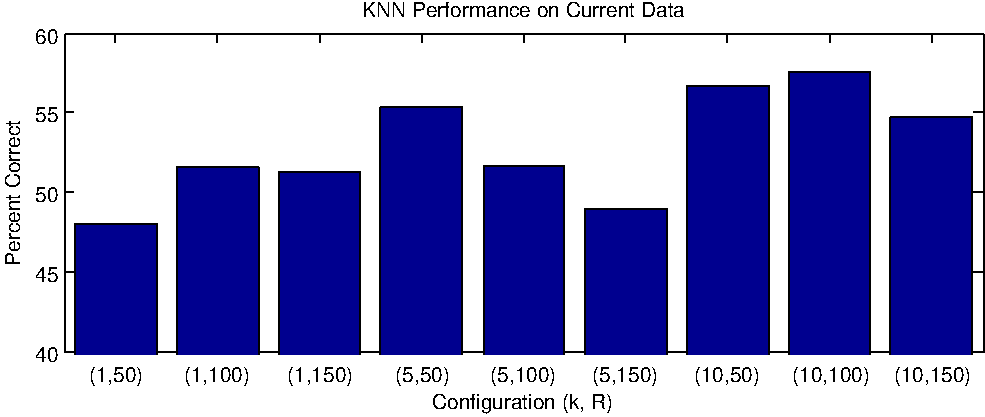
\includegraphics[scale=0.5]{plots/knn-today.pdf}
\caption{Comparison of K-Nearest-Neighbors performance with features from rank $R$ LSI for a bag of words from the current day. Results are average verification accuracy from k-fold cross validation.}
\label{fig:knncompare}
\end{figure}

Figure~\ref{fig:knncompare} illustrates the difference in accuracy between several different parameter choices in predicting the current day's class based on bags of phrases from that day. The parameter $k$ is the number of neighbors for majority-voting in KNN, and the parameter $R$ is the dimension of the reduction for LSI. Two trends emerge in this data. First, increased $k$ leads to increased accuracy. Since 57.43\% of the days are up days, increasing $k$ arbitrarially will converge to this result. For $k=10 \text{ and } k=1$, middle values of $R$ (between 50 and 150) tend to work best. It may be that low values of $R$ fail to include enough features, while higher values of $R$ overfit the training data. It is unknown why increasing $R$ decreases the accuracy of 5-nearest-neighbor. It may just be that increasing $R$ increases the sparsity of the data, and the $k=10$ results do not exhibit this because the effect is hidden by the extra neighbors (which bring it closer to the overall proportion of up days). We also ran KNN experiments on data scaled as mentioned in Section~\ref{sec:features}, with slightly worse results than reported in Figure~\ref{fig:knncompare}. This may be due to scaling causing everything to cluster together more, introducing new neighbors from different classes. Using yesterday's data to predict the current day produces results consistent with what has already been observed (close to the current day results, but occasionally lower). Surprisingly, using tomorrow's data to predict the current day results in much lower accuracy. For example, using $k=10$ and $R=100$ results in only 40.87\% accuracy. However, this indicates that our classifier is good at finding wrong answers, and building a predictor which does the opposite of K-Nearest-Neighbors for those parameters results in 59.13\% accuracy. This seems counterintuitive, and it may be due to a problem with the feature set reduction through LSI clustering non-similar features close together, or due to scaling the vectors incorrectly.

Applying SVMs to our data uncovered many issues with convergence similar to those experienced in previous experiments~\footnote{Namely, the 6.867 homeworks}. Setting the parameter $C$ too low can allow for too much slack and causes immediate termination, which is especially a problem since placing a decision boundary such that all data is classified as an up day results in 57.43\% accuracy on the set of all training data. Setting the $C$ parameter too high, however, biases the resulting predictor and reduces validation accuracy. We therefore take a less principled approach to which parameters we select, and instead present results from a brief exploration of the parameter space.

We trained a kernelized SVM with a radial basis function using several different bandwidth and $C$ parameters, and they all ended up classifying everything as an up day. We believe that for high bandwidths the greater proportion of up days in the training data results in a decision boundary that includes all data points. Since all points are clustered so close together (see the graphical representations of LSI features earlier), this results in the same decision for all points. Using a quadratic kernel with $C=1E9$ on the current day data resulted in a classifier that does not just choose the same value, but it only classified 51.91\% of the verification days correctly on average, which is lower than the predictors which choose only one answer. Even training on the augmented data was tricky and gave poor results. The main problem with SVMs on this data is that it is difficult to separate in a general way under any basis function. As illustrated graphically earlier, the different classes are distributed similarly with slight differences in lower dimensions. The KNN technique works somewhat because some information can be gathered from groups of nearby points, but attempting to create a decision boundary directly as SVMs do is difficult because of the distribution of the data.

From our results with these algorithms, we have strong evidence to support the hypothesis that newspaper articles can be used to classify stock market directions in general by using features that are highly dependent on the market (i.e. the articles for the day following the one we are classifying). Our results show that we can obtain some information that is useful in making future predictions in the market, particularly by using Naive Bayes and AdaBoost, but the correlation is very weak as we would expect. KNN methods show the dimensionality reduction using LSI does provide semantic information as expected, but it is either not expressive enough or not measuring the right semantic information. It is possible that our simplifying assumption that we can take a bag of words to represent an entire day is incorrect. We may have been able to obtain better results by modeling the topics within articles directly rather than through a latent model.

\subsubsection{Conclusions}

\subsection{Predicting the Dow Jones based on past trends}
\label{dj->dj}

\TODO{Fred: Add a discussion about making money to answer Q3}.

In this section we look at predicting the performance of the Dow Jones based on past trends to answer research question 2.
That is, at time $t$ we make predictions purely based on the previously observed performance of the Dow Jones, represented by the sequence $(Y^{(1)}, ..., Y^{(t-1)})$, and do not take Wall Street Journal articles into account.

As described in Section~\ref{sec:sequential-models} we have two sequential classifier.
Section~\ref{mm-eval} evaluates our M-order Markov Model classifier and Section~\ref{hmm-eval} evaluates our vanilla Hidden Markov Model classifier.

Our experimental setup is as follows.
Let $t\in{}[s,n]$, where $s$ is the starting point and $n$ is the number of training examples (days) as before.
For each $t$ we train our sequential classifiers using the performance of the Dow Jones the first $t-1$ days.
We then use the sequential classifiers to predict the maximum likelihood value of $Y^{(t)}$ using the model parameters found in training.

\begin{figure*}
\center
\hspace{0.5cm}
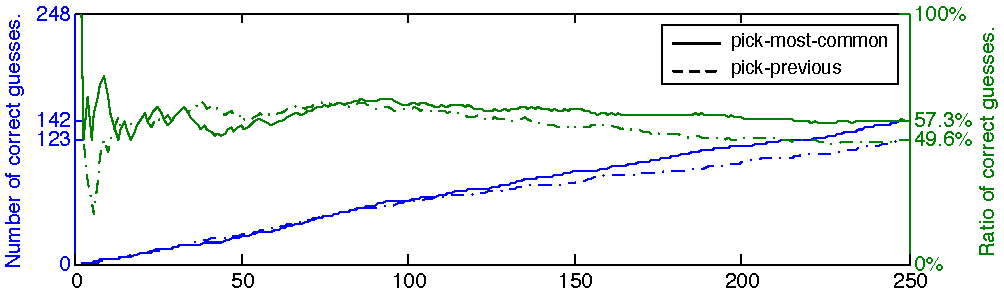
\includegraphics[width=16cm]{experiments/seq_baseline.pdf}
\caption{Plot showing two baseline heuristics. The pick-most-common heuristic predicts the direction that was most common in earlier days, while the pick-previous heuristic just predicts the same direction as the previous day. Both heuristics are plotted with accumulative number of predictions up to that day (blue), and prediction accuracy up to that day (green).}
\label{fig:seq-baseline}
\end{figure*}

We evaluated two reasonable baselines to use for comparison.
The first, called \emph{pick-most-common}, predicts each $Y_{(t)}$ to be the most common movement of the stock market for $(Y^{(1)}, ..., Y^{(t-1)})$.
The second, called \emph{pick-previous}, predicts each $Y_{(t)}$ to be the same as the preceding day.

Figure~\ref{fig:seq-baseline} shows the performance of the two baseline classifiers.
Solid lines show the performance of the pick-most-common heuristic and stippled lines show the pick-previous heuristic.
Furthermore, blue lines show the total number of correct guesses by each respective heuristic up to that day and green lines show the prediction accuracy of each heuristic up to that day.

Note that the pick-most-common classifier always predicts that the Dow Jones goes up since every prefix sequence of $Y$ is dominated by positive days. 
Note also how both predictors perform worse at the end of the year.
This is because the US was entering a recession and the market became both more negative, which caused the predict-most-common heuristic to do worse, and more volatile, which caused the predict-previous heuristic to do worse.

Since the pick-most-common heuristic for the most part dominates the pick-previous we will only use pick-most-common as a baseline in the following.


\subsubsection{Markov Models}
\label{mm-eval}

As described in Section~\ref{sec:mm} we implemented a M-order Markov Model for any M.
We ran the Markov Model on the whole sequence for $M=[1,10]$ ($w=M+1$), each time training a Markov Model on the first $t-1$ elements of $Y$ and using the resulting parameter $\theta$ to predict the value of $Y^{(t)}$.
We were able to train very high order Markov Models ($M=40$) using sparse parameter matrices.
However, for higher orders the parameter matrices is mostly empty and predictions therefore just become a tie-breaking, which is not very useful.
Figure~\ref{fig:mm-experiment} shows the aggregate prediction ratios of the Markov Models of order 1--6, together with the predict-most-common baseline.

As we can see the lower order Markov Models perform better, which is because they converge on always predicting that the Dow Jones goes up (the dominant direction). Thus they closely follow the pick-most-common heuristic once they stabilize.
However, for early predictions the Markov Model has not yet become convinced that it should predict that the Dow Jones goes up. In fact, early in 2007, when there was less market volatile that later in the year, the fourth order Markov Model is able to outperform the baseline because it finds local trends.

\begin{figure*}
\center
\hspace{0.5cm}
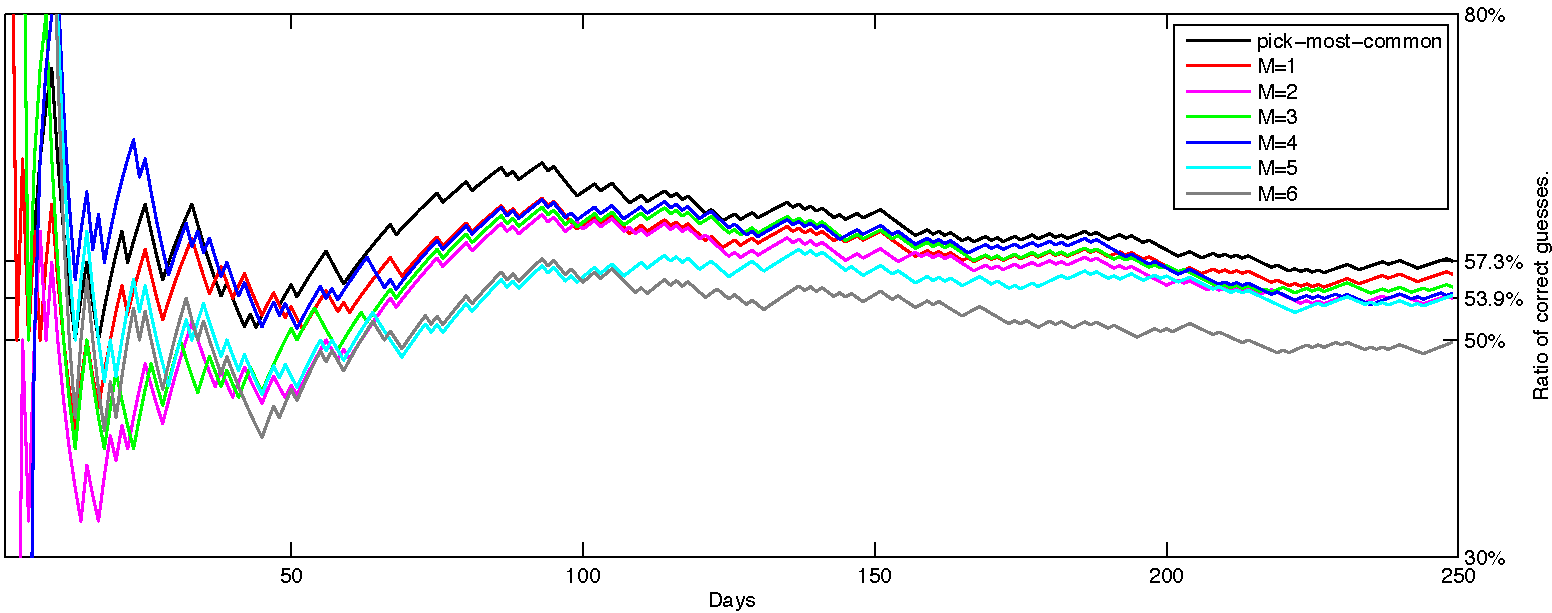
\includegraphics[width=16cm]{experiments/mm_experiment.pdf}
\caption{Plot of one through six-order Markov Models as well as the pick-most-common baseline. All plots show the prediction accuracy up to that day.}
\label{fig:mm-experiment}
\end{figure*}

\subsubsection{Hidden Markov Models}
\label{hmm-eval}

As described in Section~\ref{sec:hmm} we also implemented a Hidden Markov Model (HMM) predictor that relies heavily on MATLABs HMM toolkit for training and inference.
We ran our HMMon the whole sequence of data. For each $t$ we used all preceding observations ($Y^{(1)}$, ..., $Y^{(t-1)}$) to train our HMM and then used the HMM to predict $Y^{(t)}$.
We found that altering the initial guesses for the transition matrix A and emission matrix B didn't impact our predictions much.
However, we postulated two hidden states and made both A and B diagonal matrices with 0.6 on the diagonal.

Figure~\ref{fig:hmm-experiment} shows the HMM performance as a function of days.
The HMM predictor achieved 54.8\% accuracy on the whole dataset and thus also failed to beat the pick-most-common heuristic.
To gain some insight into why this is we also plotted the performance of the Dow Jones.
As we can see the Dow Jones follow a clear up-trend in the beginning of the year, while the last part of the year is very volatile without many longer-term downtrends.
The HMM therefore has few opportunities to get leverage on the baseline.
However, one such opportunity appears just before day 100. Here we can see that the Dow Jones falls for several days. This naturally causes the baseline's accuracy to fall, while the HMM is able to address the trend and reverse course to predicting negative days.

\begin{figure*}
\center
\hspace{0.5cm}
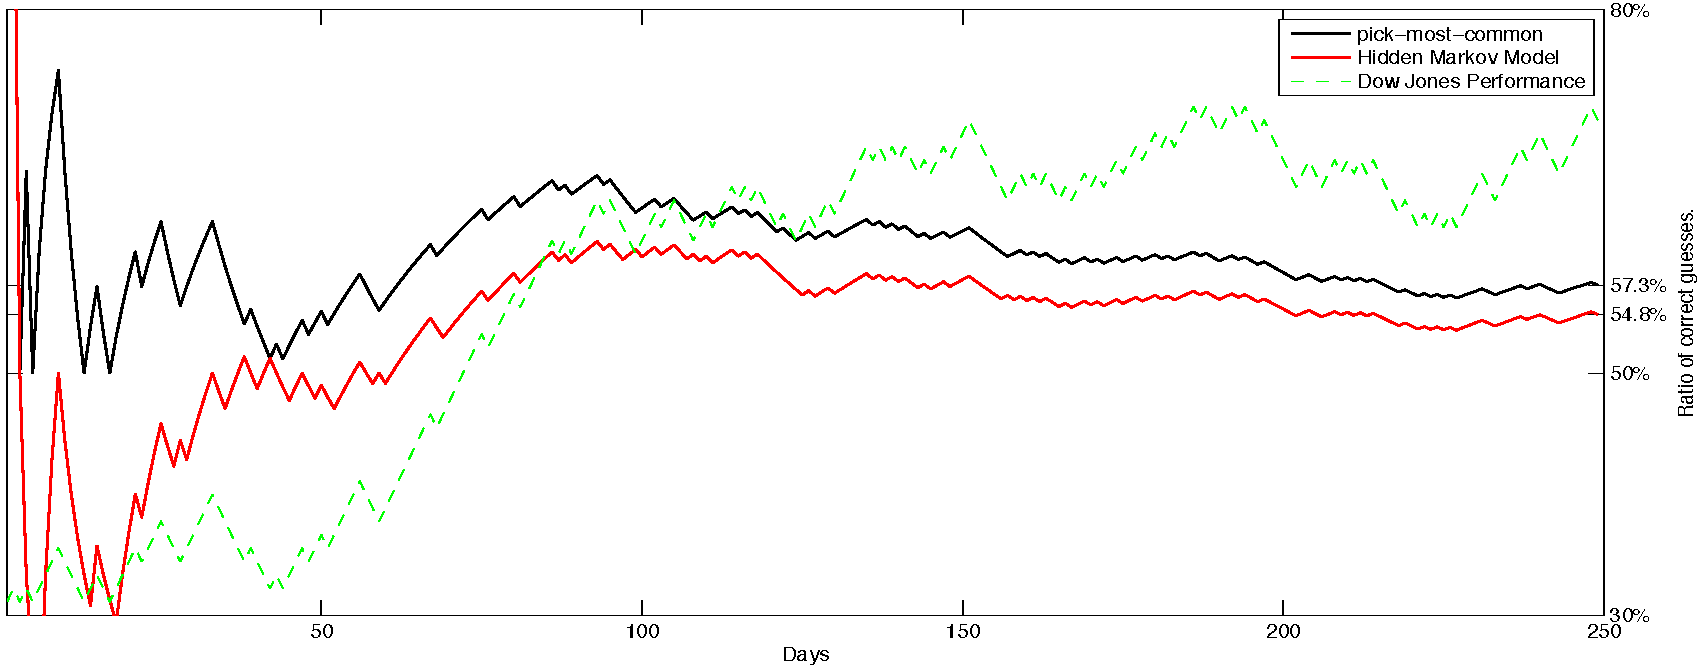
\includegraphics[width=16cm]{experiments/hmm_experiment.pdf}
\caption{Plot showing the accuracy of the baseline heuristic and the accuracy of the Hidden Markov Model. Additionally, the performance of the Dow Jones is plotted as a stippled green graph.}
\label{fig:hmm-experiment}
\end{figure*}


\subsubsection{Hidden Markov Models as priors to Naive Bayes}

\begin{figure*}
\center
\hspace{0.5cm}
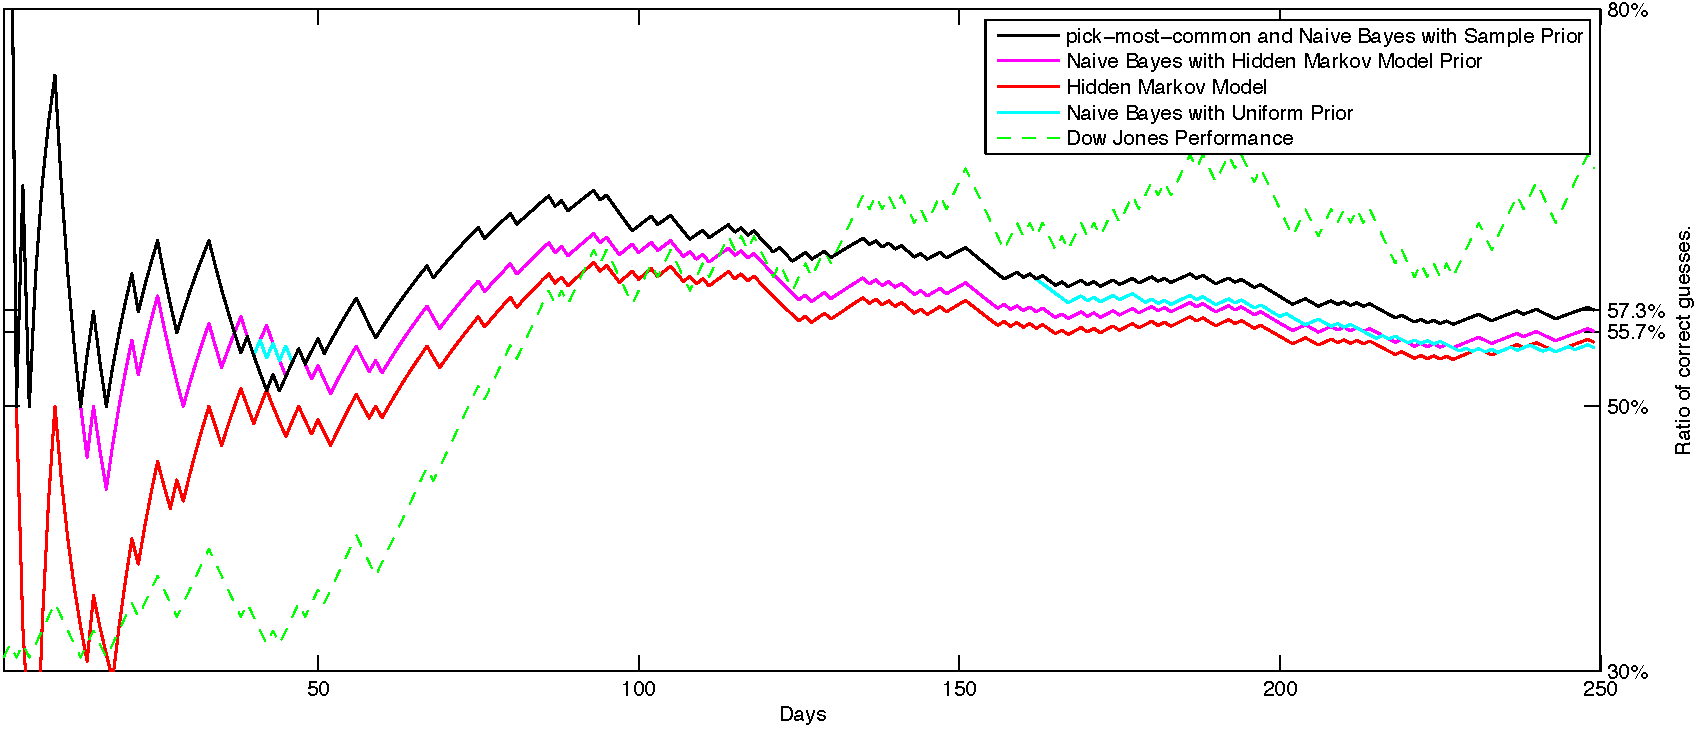
\includegraphics[width=16cm]{experiments/hmm_nb.pdf}
\caption{Plot showing the accuracy of the baseline, our Hidden Markov Model and our Hidden Markov Model where we use the marginal computed for $Y^{(t)}$ as the prior for Naive Bayes (see Figure~\ref{fig:hmm-nb-predict}). Additionally, the performance of the Dow Jones is plotted as a stippled green graph.}
\label{fig:hmm-nb-experiment}
\end{figure*}

...

Figure~\ref{fig:hmm-nb-experiment}


Two ideas for hmm-nb: normalize hmm posteriors/nb priors towards 0.5 to make them less dominant in nb, or run hmm with a relatively small window to make hmm less certain. This would give the weak signal from naive bayes a chance to win through.


\subsubsection{Conclusions}

Generally, we see that Markov Models and Hidden Markov Models perform worse than the simple pick-most-common heuristics for 2007. This is because that heuristic is pretty good for this year, with 57.4\% accuracy. Another reason is that the Dow Jones this year is very volatile and the only very significant long-term trends are positive. The heuristic naturally catches these trends, while the (Hidden) Markov Models have very few significant downward trends to use to get leverage over the baseline.

However, it is probably still better to use (Hidden) Markov Models for predicting the Dow Jones, since they will be much better able adapt to changing circumstances.
One obvious example of this would be 2008, where the US was in a severe recession and the Dow Jones fell drastically.
Here it would take a lot of time for the pick-most-common heuristics to change its mind, while especially the Hidden Markov Models would be able to turn around fast.

Finally, 2007 was a year with a lot of volatility since the US was moving into a recession.
This also helps explain why (Hidden) Markov Models, which are based on finding trends and patterns (especially local ones) in data were less effective than simple heuristics.



\section{Conclusions}

\bibliographystyle{plain}
\bibliography{report.bib}

\end{document}
